\documentclass[12pt]{article}
%\documentclass[AER]{AEA}
\usepackage{geometry}
\usepackage{enumitem}
\usepackage{float}
\setlist[itemize]{leftmargin=*}
\geometry{letterpaper}
\usepackage{float}
\usepackage{fancyhdr}
\restylefloat{table}
%% Sets page size and margins
\usepackage[margin=1in]{geometry}
\usepackage{comment}
\usepackage{caption}
\usepackage{graphicx} \usepackage{amsmath,amssymb}
\usepackage[colorlinks=true, allcolors=blue]{hyperref}
\usepackage{natbib}
\usepackage{setspace}
\usepackage{multirow}
\doublespacing
\title{Local Housing Price Nowcasting}
\author{Vittorio Garavelli, Camilla Nguyen, Lisa Collier \thanks{University of California, Berkeley, Email: vittorio.garavelli@berkeley.edu, lisa.collier@berkeley.edu, cami@berkeley.edu}}

\begin{document}
\maketitle
\vspace{-1.5cm}
\begin{abstract}
\noindent We benchmark four standard predictive approaches --- pooled OLS with metro fixed effects, ARIMA, XGBoost, and a small MLP --- on monthly Zillow Home Value Index (ZHVI) returns for three structurally different US metropolitan areas: San Francisco, Austin, and Cleveland. Predictors come from FRED macroeconomic series and Zillow listing-side variables. Models are trained on pre-2023 data and evaluated on a January~2023--March~2026 test set that covers the post-2022 mortgage-rate shock. We document two patterns. First, no single model wins everywhere: OLS is best in San Francisco, MLP is best in Austin, and ARIMA is best in Cleveland. Second, SHAP attribution on the XGBoost model shows that the most important features differ by metro. We read these results as evidence that, in the United States, both model selection and dominant features are geographically contingent.
\end{abstract}

\pagenumbering{arabic}

\section{Introduction}

Housing markets play a central role in household wealth, local economies, and monetary policy. Housing wealth represents ``one half of household net worth'' \cite{iacoviello2011}, so losses in housing wealth can dramatically decrease consumption with consequences for monetary policy and GDP growth. Predicting housing prices in real time therefore has practical value, but official indicators such as the Case-Shiller Index and the FHFA price index are published with substantial latency.

This work addresses that gap empirically. Nowcasting refers to a framework that uses real-time indicators to predict the current value of a series before its official figure is released \cite{mcgough2020}. We do not propose a new method; rather, we \emph{benchmark} four standard predictive approaches --- pooled OLS with metropolitan fixed effects, a univariate ARIMA model, XGBoost, and a two-layer MLP --- on three structurally different US metros: San Francisco (coastal), Austin (Sun Belt), and Cleveland (interior). Models are trained on pre-2023 data and evaluated on January~2023--March~2026, a window that covers the post-2022 mortgage-rate-shock regime. We ask two descriptive questions. \textbf{(i)~Do specific features emerge as the major drivers of monthly housing-price returns, or does the answer depend on the metropolitan area?} \textbf{(ii)~Is model selection itself geographically contingent in the United States?}

\section{Literature Review}
\label{sec:lit}

Our design draws on two findings in the housing-forecasting literature. \citet{rapach2009forecasting} forecast US state-level real housing price growth and document that forecastability differs sharply between interior and coastal states: autoregressive and multi-predictor models perform well for many interior states but poorly for coastal states with strong price growth. We adopt their core macroeconomic series (mortgage rate, CPI, unemployment) from FRED and extend the comparison to the metropolitan level by selecting one coastal market (San Francisco), one Sun Belt market (Austin), and one interior market (Cleveland). \citet{kholodilin2014business} forecast housing prices and rents across 71 large German cities and find that no single predictor dominates across all cities and segments; instead, the most useful indicators vary by local context. This motivates our use of \emph{both} listing-side variables (new listings, days-pending, price cuts) \emph{and} macroeconomic indicators, plus our application of SHAP attribution to identify which variables drive predictions in each metro. Our contribution is to implement metro-level housing nowcasting on three structurally different US markets, comparing classical econometric and machine-learning models on a common test set.

\section{Data}
\label{sec:data}

We use three data sources to build a monthly panel covering our three metros. The raw Zillow and FRED panel spans January~2000 to March~2026. The supervised complete-case sample begins in 2018 because the Zillow listing-side variables are unavailable before then and predictors are lagged. The OLS, XGBoost, and MLP models are trained on 168 complete pre-2023 observations and evaluated on 97 complete test observations (36 in San~Francisco, 36 in Austin, 25 in Cleveland). The ARIMA baseline is estimated separately by metro on the longer target-only ZHVI return history (back to January~2000) and aligned to the same 97-observation test grid for evaluation.

\subsection{Zillow Home Value Index}

Our first source is the Zillow Home Value Index (ZHVI), a smoothed seasonally-adjusted measure of the median home value in the middle price tier of each metropolitan area, published monthly from January~2000 onward. Alongside ZHVI we use three Zillow listing-side variables (new listings, median days from listing to pending sale, share of active listings with a price reduction); these begin in 2018, which constrains the supervised modeling window. Figure~\ref{fig:zhvi} shows the ZHVI trajectories for the three metros.

\begin{figure}[H]
\centering
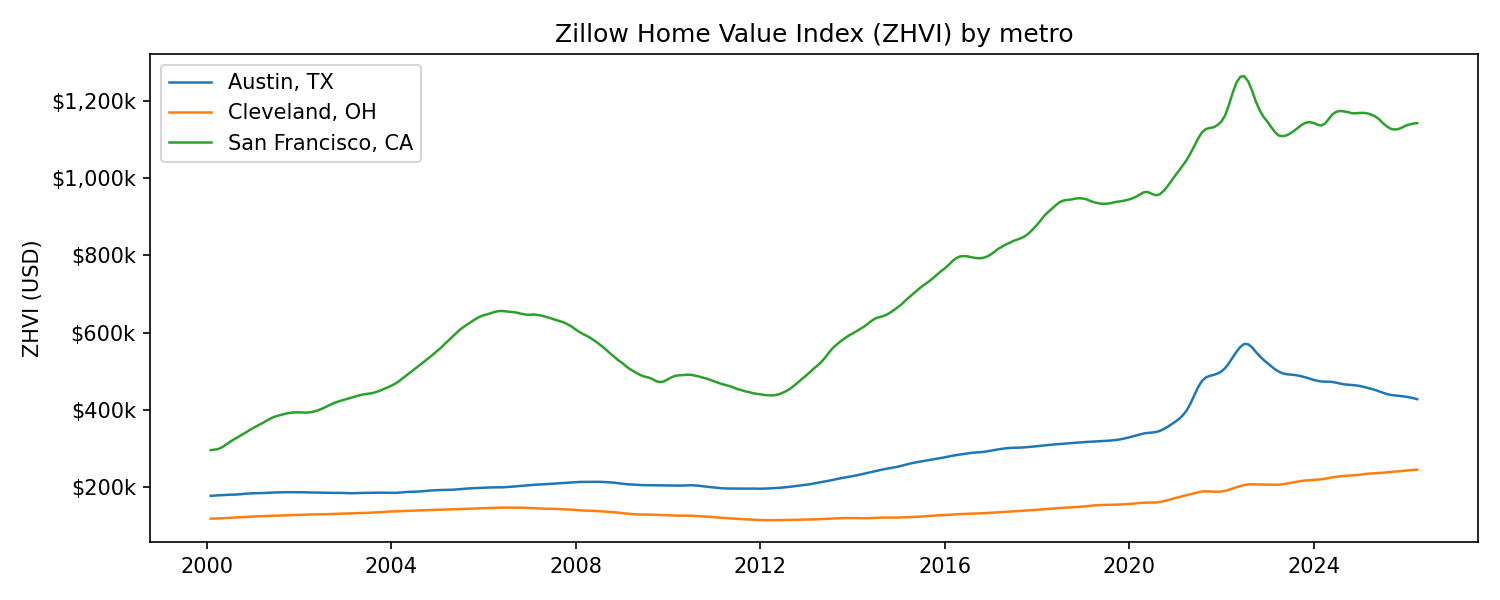
\includegraphics[width=\textwidth]{zhvi_levels.png}
\caption{Zillow Home Value Index, by metro, January 2000 to March 2026. San Francisco and Austin experience steep price growth and increased volatility compared to Cleveland.}
\label{fig:zhvi}
\end{figure}

\subsection{National and Metro Macroeconomic Indicators}

We pull five national series from the Federal Reserve Bank of St. Louis (FRED): the 30-year mortgage rate (proxying buyer affordability), the national unemployment rate, CPI (inflation), housing starts (supply-side proxy), and the St.~Louis Fed Financial Stress Index. Weekly series are resampled to monthly means. To capture local labor-market conditions, we add metro-specific seasonally-adjusted unemployment series from BLS LAUS via FRED: \texttt{SANF806URN} for San~Francisco, \texttt{AUST448URN} for Austin, and \texttt{CLEV439URN} for Cleveland.

\subsection{Sample Construction}

We merge the three sources into a single dataframe in which each row corresponds to one observation per city per month, broadcasting the national macro indicators across all metros. After dropping rows with missing listing-side values, the supervised panel contains 168 training observations (pre-2023) and 97 test observations (36 / 36 / 25 for SF / Austin / Cleveland). The Cleveland test sample is smaller because the extracted Cleveland LAUS series ends in December~2024; once the one-month lag is applied to \texttt{d\_unrate\_metro}, Cleveland's last complete-case test month is January~2025. We also collected 2024 ACS 5-year metro variables (median household income, median home value, rental vacancy rate) for descriptive context, but they are not in the model matrix because they are time-invariant within each metro and therefore perfectly collinear with the metro fixed effects.

\begin{table}[H]
\centering
\small
\caption{Summary statistics by metropolitan area. ZHVI in thousands of US dollars. Log return is the monthly log return of ZHVI. Listing-side variables (new listings, price cuts) cover 2018--2026; ZHVI and log return cover 2000--2026 (315 obs/metro); metro unemployment covers 2000--2026 for SF and Austin (313 obs each) and 2000--2024 for Cleveland (300 obs). 30-yr mortgage rate is national (mean 5.21\%, std 1.39\%, range 2.68--8.52\%).}
\label{tab:summary}
\begin{tabular}{llcccc}
\hline
Metro & Variable & Mean & Std & Min & Max \\
\hline
\multirow{5}{*}{San Francisco}
  & ZHVI (\$000s)        & 716.2  & 275.3 & 294.9  & 1264.8 \\
  & Log return           & 0.0043 & 0.0093 & -0.0234 & 0.0270 \\
  & Metro unemployment   & 5.37  & 2.25  & 2.3    & 13.9   \\
  & New listings         & 3323  & 972   & 1426   & 5136   \\
  & Price cuts (\%)      & 0.151 & 0.047 & 0.061  & 0.262  \\
\hline
\multirow{5}{*}{Austin}
  & ZHVI (\$000s)        & 279.1  & 110.9 & 176.3  & 570.4  \\
  & Log return           & 0.0028 & 0.0081 & -0.0216 & 0.0509 \\
  & Metro unemployment   & 4.50  & 1.48  & 2.4    & 11.5   \\
  & New listings         & 2957  & 810   & 1567   & 4835   \\
  & Price cuts (\%)      & 0.222 & 0.078 & 0.044  & 0.370  \\
\hline
\multirow{5}{*}{Cleveland}
  & ZHVI (\$000s)        & 148.4  & 35.5  & 112.9  & 244.5  \\
  & Log return           & 0.0023 & 0.0046 & -0.0083 & 0.0179 \\
  & Metro unemployment   & 5.57  & 1.91  & 2.1    & 20.6   \\
  & New listings         & 2440  & 638   & 1326   & 3677   \\
  & Price cuts (\%)      & 0.189 & 0.039 & 0.112  & 0.273  \\
\hline
\end{tabular}
\end{table}

\section{Empirical Strategy}
\label{sec:method}

\subsection{Target Variable}

We model the monthly log return of ZHVI rather than the raw price level:
$$y_t = \ln\!\left(\text{ZHVI}_t / \text{ZHVI}_{t-1}\right).$$
Log returns are stationary (raw home values trend), put the three cities on a comparable scale (a 0.5\% monthly change is the same effect in San Francisco and Cleveland whereas a \$5{,}000 change is not), and are the standard unit in research on rates of appreciation. Throughout, ``nowcasting'' means predicting the current month's ZHVI return using indicators available at the start of that month, before the official Zillow figure is published.

\subsection{Feature Engineering}

We apply standard stationarity transforms: first-difference the mortgage rate and the two unemployment series; log-transform new listings, housing starts, and days on market and then first-difference (denoted \texttt{d\_log\_*}); express CPI as a 12-month log change. The financial-stress index and the share of price cuts are already bounded and kept as-is.

To prevent look-ahead bias, the eight leading indicators (the differenced mortgage rate, the two unemployment changes, the three Zillow listing-side variables, the financial-stress index, and the log change in housing starts) are shifted back one month. CPI year-over-year inflation (\texttt{cpi\_yoy}) is kept contemporaneous because the 12-month moving signal is highly persistent and the lag-zero/lag-one difference is economically negligible. Finally, we one-hot-encode the metro identifier into three binary indicators that absorb time-invariant differences in price level, income, and supply structure across the three metros.

\subsection{Train / Test Split}

We use a single chronological split: observations through December~2022 form the training set, and observations from January~2023 onward form the test set. The split point is set so that the test period covers the regime immediately following the largest rise in mortgage rates in four decades, ensuring that training and test periods operate under substantially different macroeconomic conditions.

\subsection{Models}

We compare four predictive models of increasing complexity, all evaluated on the same test set. \textbf{OLS} is a pooled ordinary least squares regression estimated across the three cities with metro fixed effects (additive intercept shifts), serving as the linear baseline. \textbf{ARIMA} is an AIC-selected model fit per metro on target-only history, yielding ARIMA(4,\,0,\,9) for Austin, ARIMA(1,\,0,\,7) for San~Francisco, and ARIMA(9,\,0,\,7) for Cleveland. \textbf{XGBoost} is a gradient-boosted ensemble of shallow trees (\texttt{n\_estimators=500}, \texttt{max\_depth=4}, \texttt{learning\_rate=0.05}, \texttt{subsample=0.8}, \texttt{colsample\_bytree=0.8}, \texttt{reg\_lambda=1.0}). \textbf{MLP} is a two-layer feed-forward network with 16 and 8 ReLU units, L2 weight decay $\alpha=0.1$, and standardized inputs and target via \texttt{StandardScaler} to prevent extrapolation outside the training distribution.

\subsection{Evaluation Metrics}

We use two metrics: the mean absolute error on log returns (directly comparable across cities) and a dollar MAE that translates errors into dollars per month, $\text{Dollar MAE} = \frac{1}{n}\sum_{t} \text{ZHVI}_{t-1} \cdot |\exp(\hat{y}_t) - \exp(y_t)|$. We additionally compute SHAP feature attributions on the XGBoost model to identify which variables drive predictions in each metro on the test set.

\section{Results}
\label{sec:results}

\subsection{Model Comparison}

We evaluate all four models on the same complete-case test set (January~2023--March~2026): 36 test observations in San~Francisco and Austin and 25 in Cleveland. Tables~\ref{tab:dollar_mae} and \ref{tab:logmae} report the dollar MAE and log-return MAE respectively, and Figure~\ref{fig:preds} plots model forecasts against actual log returns.

\begin{table}[H]
\centering
\caption{Dollar MAE by model and metro (USD per month, test period 2023-01 to 2026-03). Bold indicates the best per metro.}
\label{tab:dollar_mae}
\begin{tabular}{lrrrr}
\hline
Metro & OLS & ARIMA(AIC) & XGBoost & MLP(16,8) \\
\hline
San Francisco, CA & \textbf{\$3{,}898} & \$5{,}660 & \$4{,}210 & \$5{,}219 \\
Austin, TX        & \$2{,}574 & \$2{,}371 & \$3{,}494 & \textbf{\$2{,}286} \\
Cleveland, OH     & \$748     & \textbf{\$491} & \$549 & \$1{,}064 \\
\hline
\end{tabular}
\end{table}

\begin{table}[H]
\centering
\caption{Mean absolute error on log returns by model and metro (test period 2023-01 to 2026-03). Bold indicates the best per metro.}
\label{tab:logmae}
\begin{tabular}{lrrrr}
\hline
Metro & OLS & ARIMA(AIC) & XGBoost & MLP(16,8) \\
\hline
San Francisco, CA & \textbf{0.00339} & 0.00497 & 0.00368 & 0.00455 \\
Austin, TX        & 0.00555 & 0.00518 & 0.00748 & \textbf{0.00488} \\
Cleveland, OH     & 0.00339 & \textbf{0.00226} & 0.00253 & 0.00487 \\
\hline
\end{tabular}
\end{table}

\begin{figure}[H]
\centering

\includegraphics[width=\textwidth]{predictions_vs_actual.png}
\caption{Estimated vs. actual monthly log returns of ZHVI in the test period (Jan.~2023--Mar.~2026). Black is the actual series; colored lines are model forecasts.}
\label{fig:preds}
\end{figure}

No single model wins across all three markets. In San~Francisco, pooled OLS produces the best performance at \$3{,}898 per month, outperforming both non-linear models. In Austin, MLP achieves the lowest dollar MAE at \$2{,}286 per month, with ARIMA a close second at \$2{,}371 (a margin under \$100). In Cleveland, MLP produces its worst performance at \$1{,}064 per month, while ARIMA is most convincing at \$491 per month. These patterns demonstrate that model performance is geographically contingent.

\subsection{SHAP Feature Importance}

To identify which variables drive XGBoost predictions in each metro,\footnote{XGBoost results are reproducible on the local environment used here (xgboost 3.2.0, macOS) but can drift by a few percent on different platforms (e.g., Google Colab) due to multi-threaded floating-point reduction order and version-dependent default tree methods. OLS, ARIMA, and MLP are platform-stable.} we compute SHAP values over the test set and average absolute contributions by metro (Table~\ref{tab:shap}). Three patterns emerge. In \textbf{Cleveland}, \texttt{price\_cuts} carries the most weight (mean $|\text{SHAP}|=0.0039$), followed by \texttt{d\_log\_days\_pending} ($0.0011$), while housing starts are nearly irrelevant ($0.0002$); this is consistent with a friction-sensitive, supply-constrained market in which transaction signals dominate. In \textbf{Austin}, \texttt{price\_cuts} alone is roughly five times more influential than any other variable, fitting Austin's volatile, demand-driven market where seller behavior is more informative than national macro series. In \textbf{San~Francisco}, the metro indicator carries most of the weight ($0.0028$), followed by \texttt{price\_cuts} ($0.0018$) and \texttt{d\_mortgage30} ($0.0011$), suggesting that structural characteristics of the Bay Area (income distribution, price level) explain more of the monthly variation than any single time-varying indicator.

\begin{table}[H]
\centering
\caption{Mean absolute SHAP values by feature and metro (XGBoost, test set). Higher values indicate greater average contribution.}
\label{tab:shap}
\begin{tabular}{lrrr}
\hline
Feature & San Francisco & Austin & Cleveland \\
\hline
\texttt{price\_cuts}           & 0.00180 & \textbf{0.00662} & \textbf{0.00391} \\
\texttt{metro\_San Francisco}  & \textbf{0.00279} & 0.00125 & 0.00122 \\
\texttt{d\_mortgage30}         & 0.00114 & 0.00088 & 0.00084 \\
\texttt{d\_log\_days\_pending} & 0.00086 & 0.00067 & 0.00110 \\
\texttt{d\_log\_new\_listings} & 0.00085 & 0.00063 & 0.00081 \\
\texttt{stlfsi}                & 0.00078 & 0.00071 & 0.00053 \\
\texttt{cpi\_yoy}              & 0.00046 & 0.00098 & 0.00053 \\
\texttt{d\_log\_houst}         & 0.00022 & 0.00020 & 0.00019 \\
\hline
\end{tabular}
\end{table}

\section{Discussion}

Our findings echo the core result of \citet{kholodilin2014business}, who document that no single predictor dominates across all German cities; we observe an analogous pattern for \emph{model architectures}, with no single nowcasting model outperforming the others across all three metros. Each model outperforms in a specific geographical area, so the optimal model type depends on the structural and macroeconomic characteristics under which a local housing market operates.

\subsection{Limitations}
Several limitations constrain our findings. The missingness of Zillow listing-side variables before 2018 limits the supervised training window to 168 complete observations, which raises overfitting risk for XGBoost and MLP; we mitigate this with conservative hyperparameters (shallow trees, heavy L2 regularization), but a longer historical record would let these models exploit more of their capacity. Second, ARIMA is estimated once on the training series and produces predictions for the full test period without updating; a rolling re-estimation scheme would more accurately reproduce real-time conditions and likely improve ARIMA performance.

\subsection{Policy Implications}
The strong performance of listing-side data across all three cities suggests that publicly available Zillow indicators can meaningfully improve price nowcasting. For policy purposes, locally calibrated nowcasting models will outperform any attempt at a universal model.

\section{Conclusion}
This paper contributes to the housing-nowcasting literature by demonstrating that model selection and feature importance are geographically contingent rather than universal. We extend prior findings along two dimensions: we develop the framework at the metropolitan level using real-time listing-side data, and we apply SHAP feature attribution to quantify precisely which variables drive each model's performance in each local market. Future work could incorporate higher-frequency data, apply rolling re-estimation to the ARIMA baseline, or expand the metro sample to test whether the geographic heterogeneity we document generalizes beyond our three chosen markets.

\section{AI Usage Disclosure}

We used Anthropic's Claude (Opus 4.6 Max and 4.7 Max) via the Claude Code CLI (\href{https://github.com/anthropics/claude-code}{github.com/anthropics/claude-code}) as a coding assistant, together with skills/agents from two open-source collections: the Everything Claude Code plugin (\href{https://github.com/affaan-m/everything-claude-code}{github.com/affaan-m/everything-claude-code}) and Scientific Agent Skills (\href{https://github.com/K-Dense-AI/scientific-agent-skills}{github.com/K-Dense-AI/scientific-agent-skills}). The model supported code review, design-weakness brainstorming (look-ahead bias, sample-size constraints, residual autocorrelation), and visual-style consistency across figures, but not the framing of the research question or the economic conclusions. Every suggested edit was reviewed manually, the notebook was re-run end-to-end after each substantive change, and all numerical results were verified against simple baselines.

\bibliography{Bibliography}
\bibliographystyle{plainnat}

\end{document}
